\documentclass[10pt,a4paper]{article}
\usepackage[utf8]{inputenc}
\usepackage{amsmath}
\usepackage{amsfonts}
\usepackage{amssymb}
\usepackage{pdfpages}
\usepackage{graphicx}
\usepackage[varg]{txfonts}
\begin{document}
\title{Problems for Tutorial-02: Scientific Plotting}
\date{}
\maketitle
\begin{enumerate}
\item Write a Scilab script to plot the data in Tut2Problem.csv. 
The first column is the x-axes data. Use proper legends and labels.
(If required use semilog/loglog plot).
\item Save a print quality pdf file of the figure generated. Name the 
file \verb'Tut2fig1.pdf'.
\end{enumerate}
{\bf Solution:} This is a semilog plot.
\begin{figure}[ht!]
\centering{
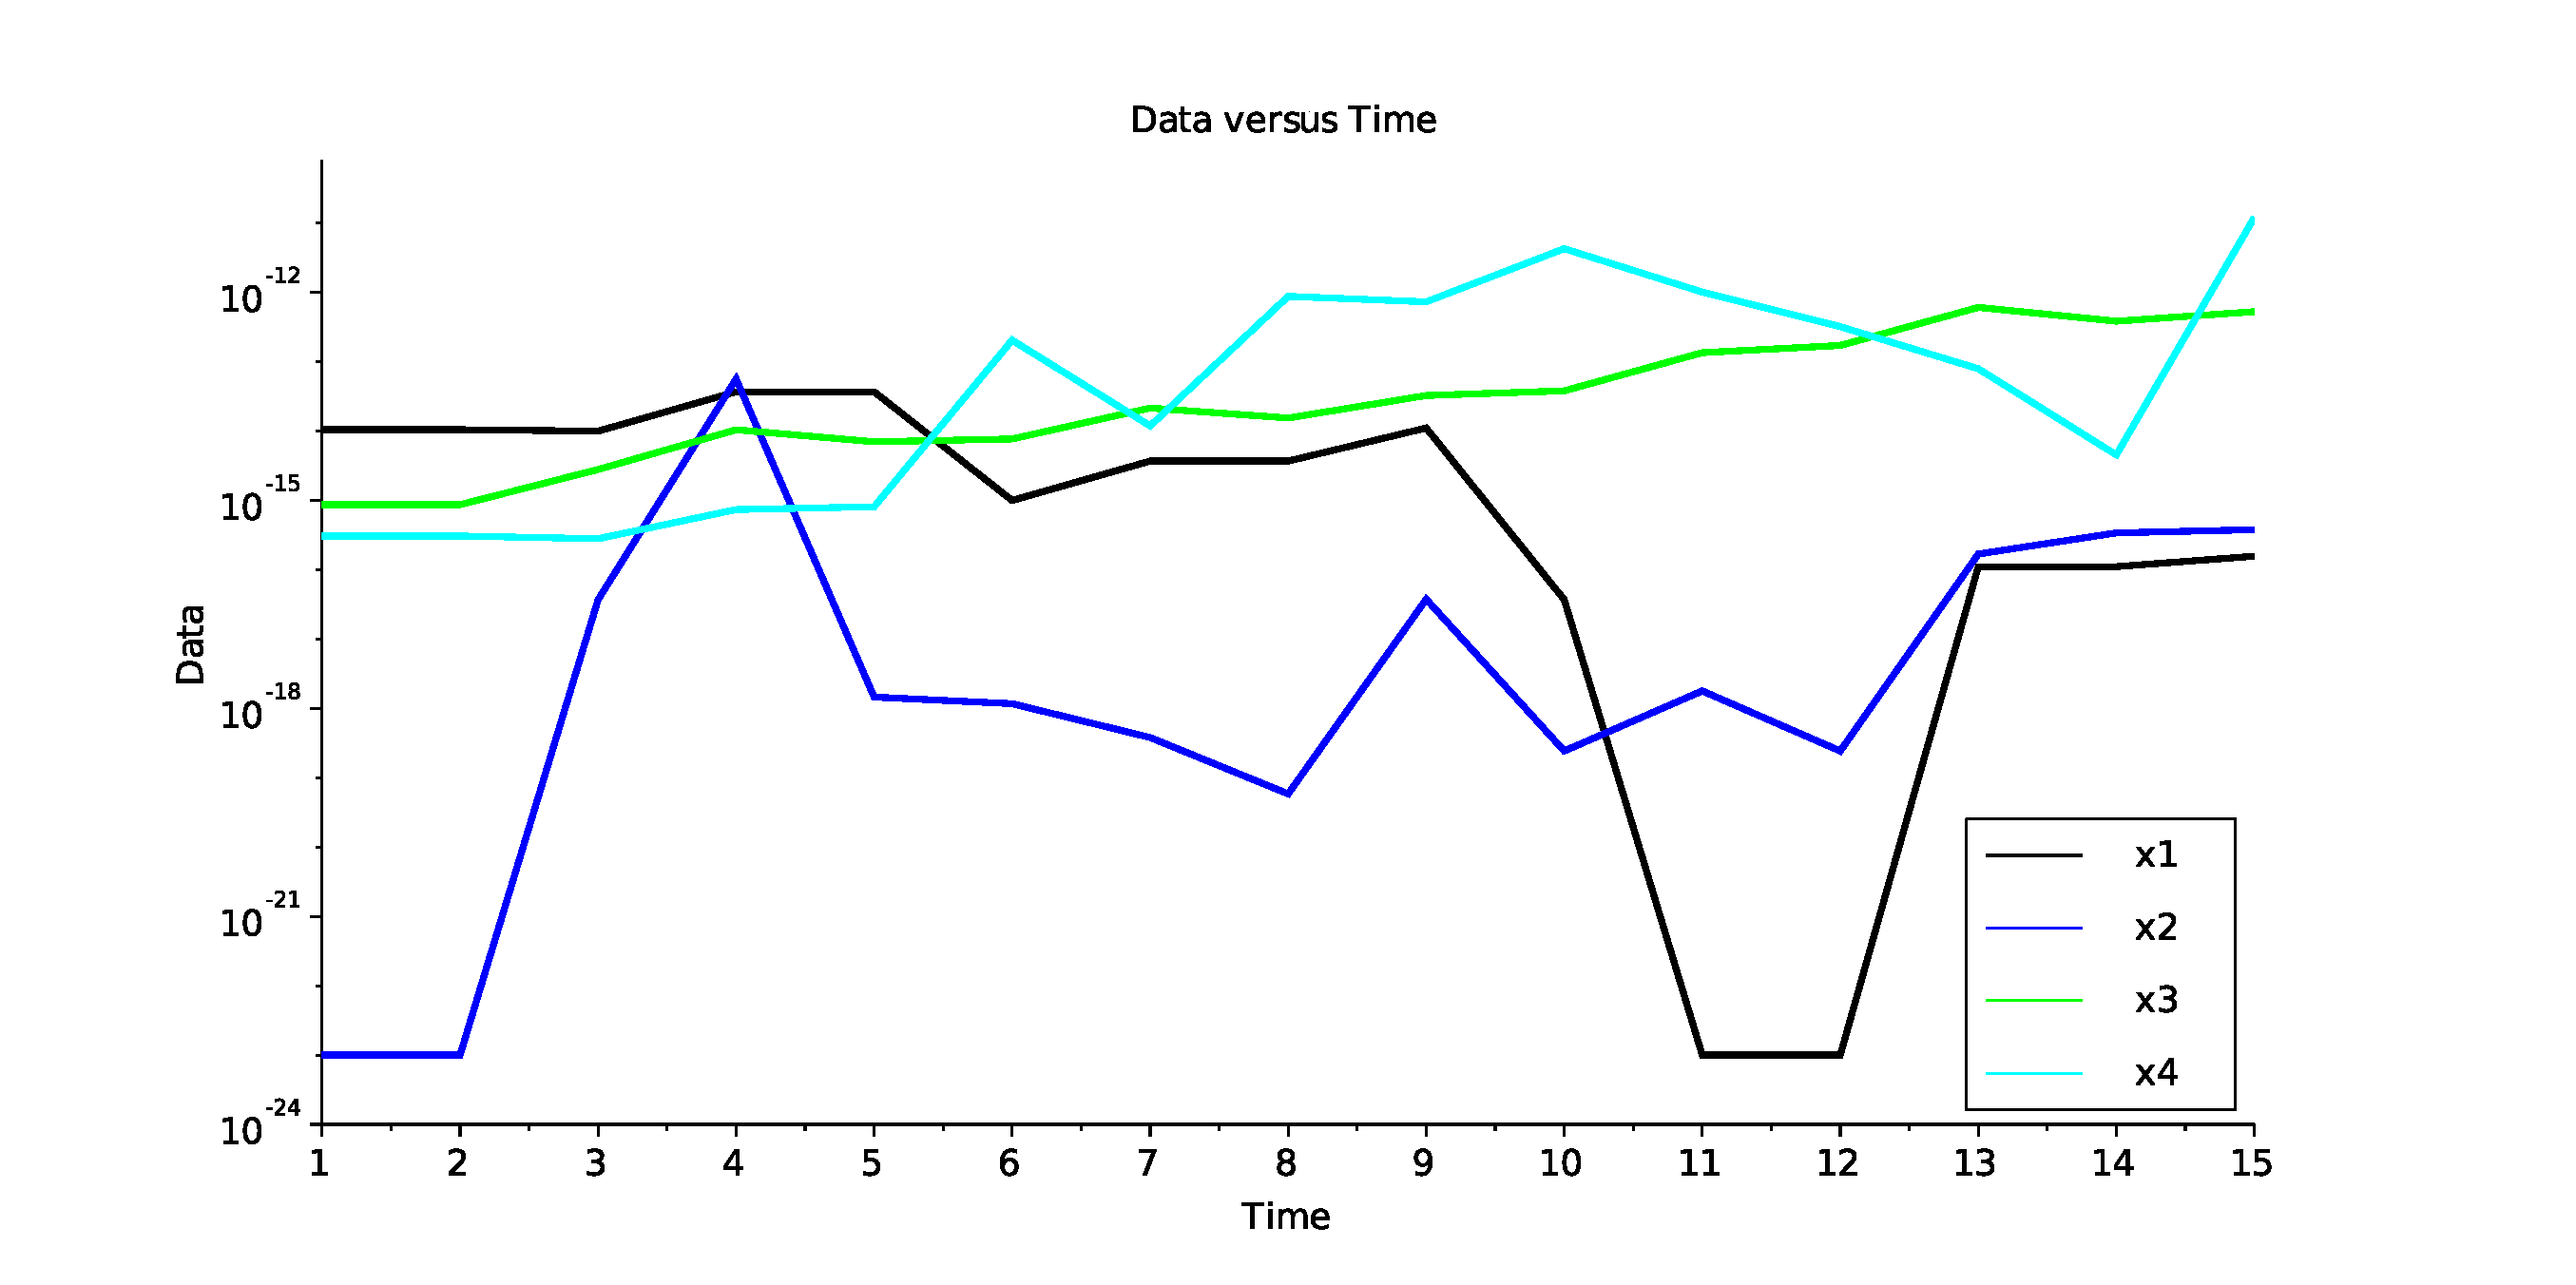
\includegraphics[scale=0.31]{SolPrblm2.pdf}}
\end{figure}
\end{document}
